%\section{Implementation and detailed design}
\chapter{Implementation and detailed design}

Present implementation details, program structure etc.

Further, interesting algorithms and data structures should be presented here.

\section{Gameloop}
dTime...

\section{Actors}
\subsection{Hero}
Movement
\subsection{Enemies}
AI
Types

\subsection{Logic}
Attacks

\section{Scenes}
Scenes keep a linked list of currently all active props and units.
Also has an array of minotaurs to be reused.
The map is just a two-dimensional array of Tiles. Tiles is an enum, where each tile is a byte, so it is an array of bytes.
\subsection{Generator} %Carsten
Map generation is executed at setup and whenever the game ends (either by player death or win). The method {\tt newScene} generates a new map with matching points at the entrance and exits. Arduino's programming language does not support returning more than one value, so the method manipulates given pointers instead like in C programming. The new map data overwrites the old one to save time and space, so the given {\tt scene} argument is a pointer to the old scene. Reusing it saves us from instantiating a new one and deallocating the old one. We ar not interested in reusing the actual map data, since the player cannot revisit prior levels.\\
The actual algorithm is in three parts: clearing, modulation and generation. First it clears the old map data, setting all tiles to {\tt NONE}, to make sure nothing is left over from the old map. This may be a bit expensive on the processing time considering it is superfluous if the generator works correctly. The reason is a design choice which will be apparent when we reach the generation.\\ %Picture of Modules?
Modulation in this case means separating the map into \emph{modules}\footnote{As opposed to vary the pitch in a voice}. This is where the layout of the map is decided. A module is a small map in itself, in our case a 5x5 map of tiles. These have been designed by hand and hard-coded into the generator. Every map is construed of a grid of modules, in our case 4x4. The modules are differentiated by which sides one can access it from. By this we mean the player can traverse from and to this module from the given sides. The types are left-right (corridor), left-right-up (T-up), left-right-down (T-down), all (cross) and none (closed). A module in the category left-right is guaranteed to have an exit left and right, and may have an exit up or down.\\
The algorithm first instantiates a grid of empty modules, and randomly assigns one of the bottom modules to be a corridor and the entrance. This is the beginning of the solution path, which guarantees that the map can be completed by the player. From then on it picks a direction, left or right, randomly. From then on the algorithm randomly either moves according to its direction or up. When moving sideways the newly visited grid space is assigned to be a corridor. If it hits the edge of the map it moves upwards and changes direction instead. Whenever the solution path moves upwards, the algorithm has to change the space it is in first. If it is in a corridor tile, it changes it to a T-up, and if it is a T-down it changes it to a cross module. Both of these are the same as their predecessors, but with a guaranteed top-side exit. The newly visited module is assigned a T-down module. The algorithm picks a new direction at random (only if it is not at an edge.) and can start the over again. When it attempts to move upwards while at the top, it instead places the exit in the current tile and terminates. All unvisited grid spaces are assigned closed modules, and are not part of the solution path. Thus we have reached a map which has a guaranteed solution.\\
Lastly the program generates the map. This step reads each module in the newly generated grid, randomly picks a module of the specified type, and fills it into the actual map. If it is currently in an entrance or exit room, it places the corresponding door. It changes the original given entrance and exit pointers to point at the now created door.\\
Every module overlap with a single row or column with all surrounding modules. Overlapping follows a priority of tiles, where the algorithm determines which tile from the modules is used. Platforms are placed before empty tiles, and solid tiles are placed before platforms. This has several benefits. Firstly the maps are more unique since pairs of modules also differ, and makes the seams of modules harder to notice. Secondly, it ensures that upward exits are easier guaranteed since platforms can be placed closer to the upper floors. This is the reason we need to clear the map prior to generation: the old tiles would disrupt this priority, since the algorithm would not be able to discern what is old and what is new during generation.\\
Old version (nondeterministic time)
\section{Optimization}
Unused functions

Data Types
Getters/Setters
Repeated statements

\subsection{Code Size bloat}
Bootloader
GD2
includes

\subsection{Further optimization}
Custom written or shortened extern libraries

%\section{Game loop}
%Essentially the game is one long loop, which ends whenever the game does. Each iteration executes the gamelogic per frame, such as moving the player and monsters around. Gameloops vary from simple while(true) loops to dynamic separate gameloops handling separate calculations (such as separating rendering from gameplay).For this we only needed a simple game loop, updating the world in each iteration. To ensure a consistent gameplay experience, we needed to know how much time passes betweenframe updates. Without this, the game would run faster or slower on different processors or inconsistently in different ingame events, throwing off the players’ sense of timing. For example, the game would be equally playable with either 30 or 60 frames per second. If the difference isn’t incorporated in the gamelogic though,the game would run twice as fast with 60 frames per second! Our implementation of a frames per second counter, is simply calculating how many frames was calculated the last frame, and then assuming the next frame has the same amount. This is a pretty simple solution, which could easily be expanded upon if needed. The obvious criticism of this method, is that the frame calculations between each second are not accounted for, and that the framerate is essentially a second behind any framerate changes.

%\subsection{Movement}
%The movement of our hero will mainly be right and left. He will have also have the ability to jump. Beside the basics movements, our hero will also have fight moves. The fight moves contains moves like sword swinging and archery.

\section{Input}
The Gameduino 2 comes with a touch screen and accelerometer. These modules gives us an opportunity to interact with the game in many ways. We could use the accelerometer or the screen to move the hero. We don’t have much experience with the screen and its capabilities. Therefore another option as backup is preferable.\\
Another option will be using an external controller. The Wii nunchuck is popular and is very suitable for this game.  Using the buttons we game can be controlled as seen in the figure below.

\begin{figure}[h]
  \centering
  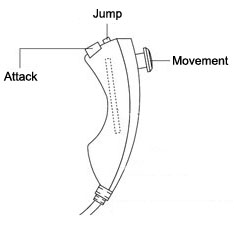
\includegraphics[scale=0.6]{Figures/nunchuk}
  \caption{Button specifications}
\label{fig:Nunchuk}
\end{figure}
